\documentclass[UTF8]{ctexart}
\usepackage{bm}
\usepackage{amssymb}
\usepackage{mathtools}
\usepackage{amsmath}
\usepackage{float}
\usepackage{booktabs}
\title{\heiti 最优化第三次作业}
\author{\kaishu 张晋15091060}
\begin{document}
\maketitle
\begin{enumerate}
\item[2.8] 设该基本可行解$\bm{x}$为$x_1,x_2,\cdots,x_n$,
其中$x_1,x_2,\cdots,x_m$为其基本可行解的基,对于$z(\bm{x})=\bm{c}^T\bm{x}=z_0+r_{m+1}x_{m+1}+,\cdots,+r_nx_n=z_0$,$z$在该基本可行解下取到下界$z_0$.若存在其他解$\bm{x}'$,则$z(\bm{x}')=z_0+r_{m+1}x_{m+1}'+,\cdots,+r_nx_n'$,
在$x_{m+1}',x_{m+2'},\cdots,x_n'$中至少有一个大于0,否则$\bm{x}'=\bm{x}$.

$\because r_j,x_j'>0 \quad \forall m+1\leq j \leq n.\quad \therefore z(\bm{x}')>z_0=z(\bm{x})$,即不存在其他最优解.

\item[2.9] 举例如下:
\begin{alignat}{2}
min \quad & x_1 \nonumber\\
\mbox{s.t.}\quad
&x_1+x_2-x_3=1 \nonumber\\
&-x_2+x_3=0 \nonumber \\
&x_i\geq 0\quad(i=1,2,3)
\end{alignat}

显然该最优解在$x_1=1,x_2=x_3$时取到。
其单纯形表如下:
\begin{table}[H]
\centering
\caption{2.9题例的单纯形表}
	\begin{tabular}{ccccc}
	\toprule
	{}&$x_1$&$x_2$&$x_3$&$b$\\
	\midrule
	{}&1&1&-1&1\\
	{}&0&-1&1&0\\
	$\bm{r}^T$&-1&0&0&0\\
	\bottomrule
	\end{tabular}
\end{table}

虽然$\bm{a}_1$对应的$r_1<0$,但对应的可行解$(1,0,0)^T$为最优解.
\item[2.10] 化为标准形如下:
\begin{alignat}{2}
min \quad & x_1-x_2 \nonumber\\
\mbox{s.t.}\quad
&x_1-x_2+x_3=2 \nonumber\\
&x_1+x_2+x_4=6 \nonumber \\
&x_i\geq 0\quad(i=1,2,3,4)
\end{alignat}

\begin{table}[H]
\centering
	\begin{tabular}{cccccc}
	\toprule
	{}&$x_1$&$x_2$&$x_3$&$x_3$&$b$\\
	\midrule
	{}&1&-1&1&0&2\\
	{}&1&\boxed{1} &0&1&6\\
	$\bm{r}^T$&1&-1&0&0&0\\
	\bottomrule
	\end{tabular}
	\caption{第一次迭代}
\end{table}
取1为转轴元,此时解为$(0,0,2,6)^T$
\begin{table}[H]
\centering
	\begin{tabular}{cccccc}
	\toprule
	{}&$x_1$&$x_2$&$x_3$&$x_3$&$b$\\
	\midrule
	{}&2&0&1&1&8\\
	{}&1&1 &0&1&6\\
	$\bm{r}^T$&2&0&0&1&6\\
	\bottomrule
	\end{tabular}
	\caption{第二次迭代}
\end{table}

此时得最优解为$(0,6,8,0)^T$,即在$x_1=0,x_2=6$时得原问题最优值为6.
$x_1,x_2$空间的可行域见图1,单纯形法的解从$(0,0)$迭代到$(0,6)$
\begin{figure}[H]
\small
\centering
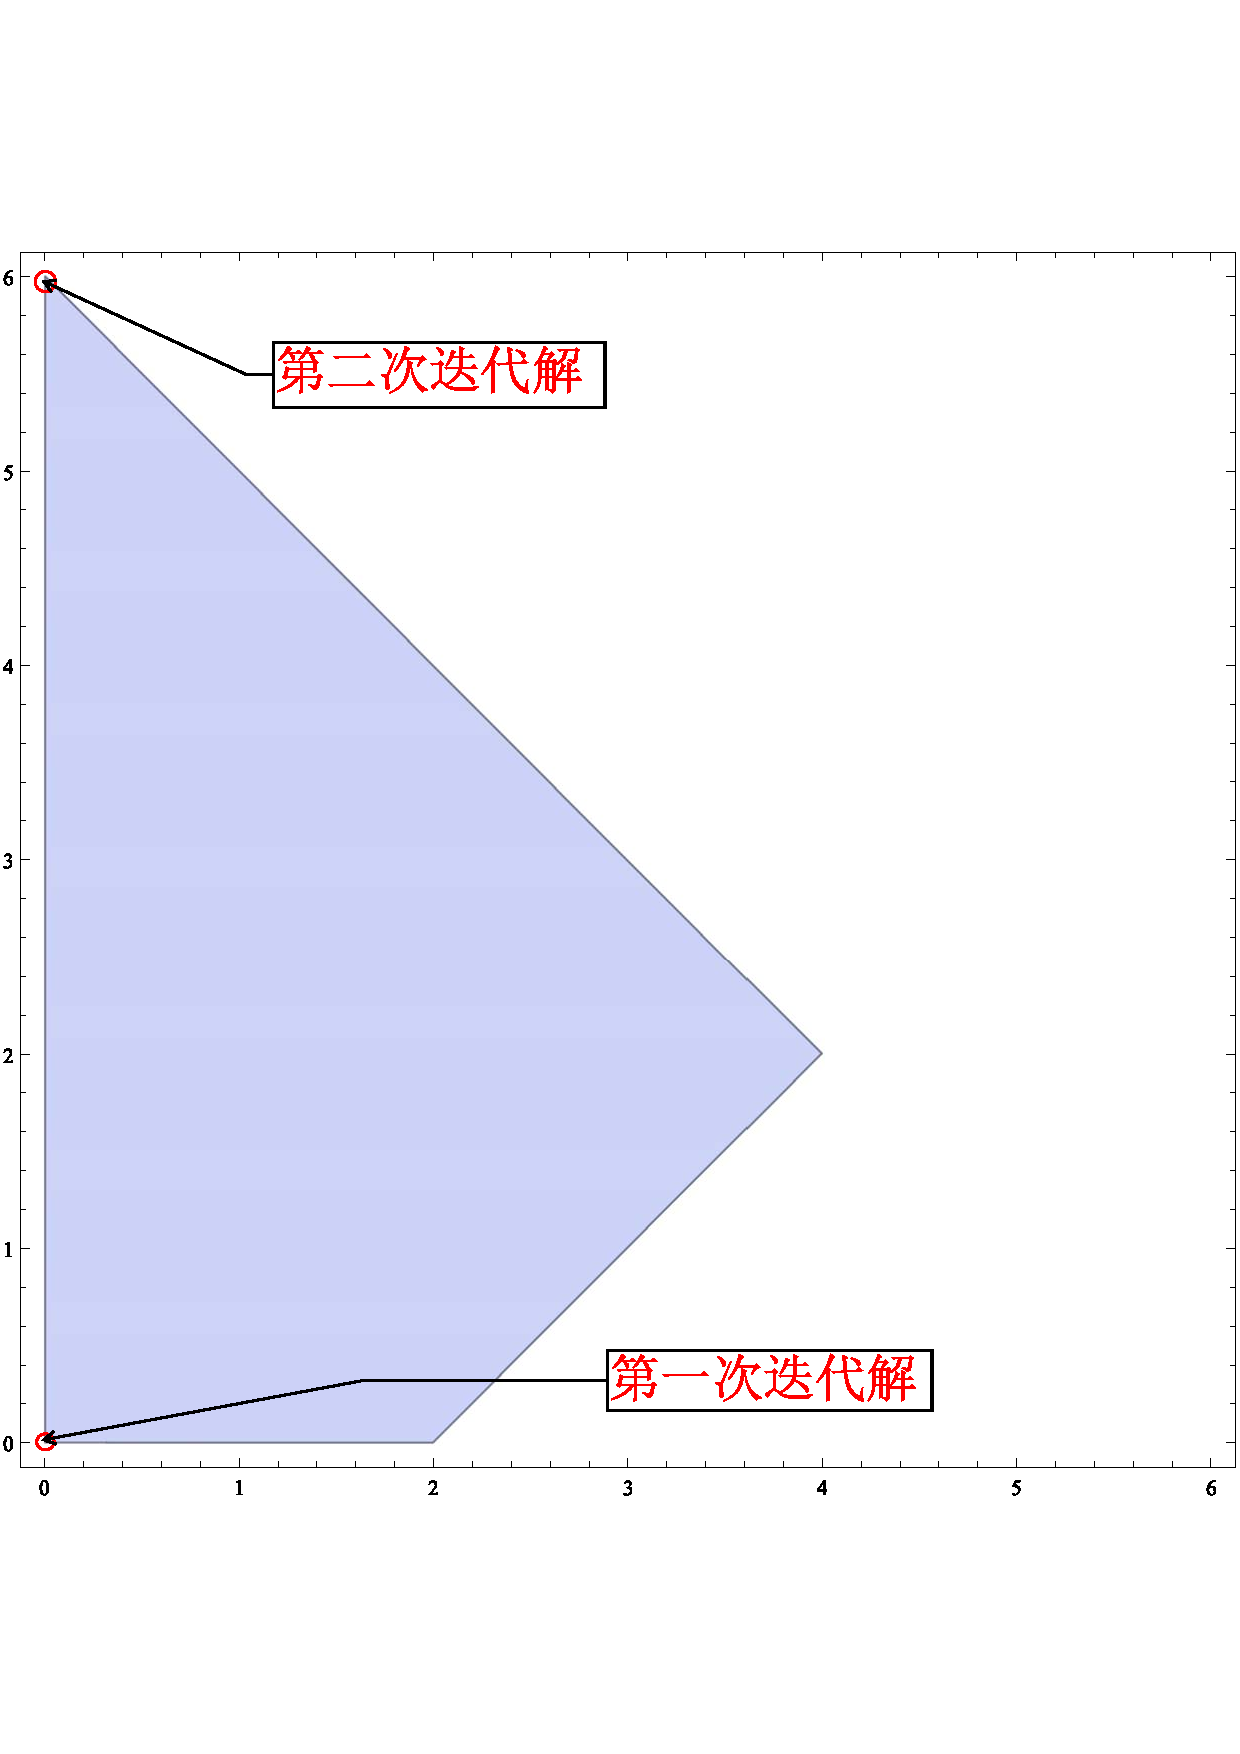
\includegraphics[width=12cm]{flow2.pdf}
\caption{可行域图}
\label{fig:1}
\end{figure}

\newpage
\item[2.20] 单纯形表如下:

\begin{table}[H]
\centering
	\begin{tabular}{cccccccc}
	\toprule
	{}&$x_1$&$x_2$&$x_3$&$x_4$&$x_5$&$x_6$&$b$\\
	\midrule
          {}&\boxed{ 1}     & 0     & 0     & 1     & 0     & 0     & 1 \\
          {}& 4     & 1     & 0     & 0     & 1     & 0     & 100 \\
          {}& 8     & 4     & 1     & 0     & 0     & 1     & 10000 \\
          $\bm{r}^T$& -4    & -2    & -1    & 0     & 0     & 0     & 0 \\
	\bottomrule
	\end{tabular}
\end{table}

\begin{table}[H]
\centering
	\begin{tabular}{cccccccc}
	\toprule
	{}&$x_1$&$x_2$&$x_3$&$x_4$&$x_5$&$x_6$&$b$\\
	\midrule
          {}& 1     & 0     & 0     & 1     & 0     & 0     & 1 \\
          {}& 0     & \boxed{ 1}      & 0     & -4     & 1     & 0     & 96 \\
          {}& 0     & 4     & 1     & -8     & 0     & 1     & 9992 \\
          $\bm{r}^T$& 0    & -2    & -1    & 4     & 0     & 0     & 4 \\
	\bottomrule
	\end{tabular}
\end{table}

\begin{table}[H]
\centering
	\begin{tabular}{cccccccc}
	\toprule
	{}&$x_1$&$x_2$&$x_3$&$x_4$&$x_5$&$x_6$&$b$\\
	\midrule
          {}& 1     & 0     & 0     & \boxed{1}     & 0     & 0     & 1 \\
          {}& 0     & 1      & 0     & -4     & 1     & 0     & 96 \\
          {}& 0     & 0     & 1     & 8     & -4     & 1     & 9608 \\
          $\bm{r}^T$& 0    & 0    & -1    & -4     & 2    & 0     & 196 \\
	\bottomrule
	\end{tabular}
\end{table}

\begin{table}[H]
\centering
	\begin{tabular}{cccccccc}
	\toprule
	{}&$x_1$&$x_2$&$x_3$&$x_4$&$x_5$&$x_6$&$b$\\
	\midrule
          {}& 1     & 0     & 0     & 1     & 0     & 0     & 1 \\
          {}& 4     & 1      & 0     & 0     & 1     & 0     & 100 \\
          {}& -8     & 0     & \boxed{1}     & 0     & -4     & 1     & 9600 \\
          $\bm{r}^T$& 4    & 0    & -1    &0     & 2    & 0     & 200 \\
	\bottomrule
	\end{tabular}
\end{table}

\begin{table}[H]
\centering
	\begin{tabular}{cccccccc}
	\toprule
	{}&$x_1$&$x_2$&$x_3$&$x_4$&$x_5$&$x_6$&$b$\\
	\midrule
          {}&\boxed{1}     & 0     & 0     & 1     & 0     & 0     & 1 \\
          {}& 4     & 1      & 0     & 0     & 1     & 0     & 100 \\
          {}& -8     & 0     & 1     & 0     & -4     & 1     & 9600 \\
          $\bm{r}^T$& -4    & 0    & 0    &0     & -2    & 1     & 9800 \\
	\bottomrule
	\end{tabular}
\end{table}

\begin{table}[H]
\centering
	\begin{tabular}{cccccccc}
	\toprule
	{}&$x_1$&$x_2$&$x_3$&$x_4$&$x_5$&$x_6$&$b$\\
	\midrule
          {}&1     & 0     & 0     & 1     & 0     & 0     & 1 \\
          {}& 0     & 1      & 0     &-4     & \boxed{1}     & 0     & 96 \\
          {}& 0     & 0     & 1     & 8     & -4     & 1     & 9608 \\
          $\bm{r}^T$& 0    & 0    & 0    &4     & -2    & 1     & 9804 \\
	\bottomrule
	\end{tabular}
\end{table}

\begin{table}[H]
\centering
	\begin{tabular}{cccccccc}
	\toprule
	{}&$x_1$&$x_2$&$x_3$&$x_4$&$x_5$&$x_6$&$b$\\
	\midrule
          {}&1     & 0     & 0     & \boxed{1}     & 0     & 0     & 1 \\
          {}& 0     & 1      & 0     &-4     & 1     & 0     & 96 \\
          {}& 0     & 4     & 1     & -8     & 0     & 1     & 9992 \\
          $\bm{r}^T$& 0    & 2    & 0    &-4     & 0    & 1     & 9996 \\
	\bottomrule
	\end{tabular}
\end{table}

\begin{table}[H]
\centering
	\begin{tabular}{cccccccc}
	\toprule
	{}&$x_1$&$x_2$&$x_3$&$x_4$&$x_5$&$x_6$&$b$\\
	\midrule
          {}&1     & 0     & 0     & 1     & 0     & 0     & 1 \\
          {}& 4     & 1      & 0     &0     & 1     & 0     & 100 \\
          {}& 8     & 4     & 1     & 0     & 0     & 1     & 10000 \\
          $\bm{r}^T$& 4   & 2    & 0    &0     & 0    & 1     & 10000 \\
	\bottomrule
	\end{tabular}
\end{table}

单纯形法迭代完毕后得最优解$(0,0,10000)$,得最优值10000.

\newpage
\item[2.21]单纯形表如下:

\begin{table}[H]
\centering
	\begin{tabular}{ccccccccc}
	\toprule
	{}&$x_1$&$x_2$&$x_3$&$x_4$&$x_5$&$x_6$&$x_7$&$b$\\
	\midrule
          {}& 1     & 0     & 0     & \boxed{ 1/4}  & -8     & -1     & 9     & 0     \\
          {}& 0     & 1     & 0     &  1/2  & -12     & - 1/2 & 3     & 0     \\
          {}& 0     & 0     & 1     & 0     & 0     & 1     & 0     & 1     \\
          $\bm{r}^T$& 0     & 0     & 0     & - 3/4 & 20     & - 1/2 & 6     & 0     \\
	\bottomrule
	\end{tabular}
\end{table}

\begin{table}[H]
\centering
	\begin{tabular}{ccccccccc}
	\toprule
	{}&$x_1$&$x_2$&$x_3$&$x_4$&$x_5$&$x_6$&$x_7$&$b$\\
	\midrule
    {}    & 4     & 0     & 0     & 1     & -32     & -4     & 36     & 0     \\
    {}    & -2     & 1     & 0     & 0     & \boxed{4}     & 3/2  & -15     & 0     \\
    {}    & 0     & 0     & 1     & 0     & 0     & 1     & 0     & 1     \\
    $\bm{r}^T$ & 3     & 0     & 0     & 0     & -4     & -7/2 & 33     & 0     \\
	\bottomrule
	\end{tabular}
\end{table}

\begin{table}[H]
\centering
	\begin{tabular}{ccccccccc}
	\toprule
	{}&$x_1$&$x_2$&$x_3$&$x_4$&$x_5$&$x_6$&$x_7$&$b$\\
	\midrule
{}    & -12   & 8     & 0     & 1     & 0     &\boxed{ 8}     & -84   & 0 \\
    {}    & -1/2  & 1/4   & 0     & 0     & 1     & 3/8   & -15/4 & 0 \\
    {}    & 0     & 0     & 1     & 0     & 0     & 1     & 0     & 1 \\
    $\bm{r}^T$      & 1     & 1     & 0     & 0     & 0     & -2    & 18    & 0 \\
	\bottomrule
	\end{tabular}
\end{table}

\begin{table}[H]
\centering
	\begin{tabular}{ccccccccc}
	\toprule
	{}&$x_1$&$x_2$&$x_3$&$x_4$&$x_5$&$x_6$&$x_7$&$b$\\
	\midrule
    {}    & -3/2  & 1     & 0     & 1/8   & 0     & 1     & -21/2 & 0 \\
    {}    & 1/16  & -1/8  & 0     & -3/64 & 1     & 0     & \boxed{3/16}  & 0 \\
    {}    & 3/2   & -1    & 1     & -1/8  & 0     & 0     & 21/2  & 1 \\
    $\bm{r}^T$     & -2    & 3     & 0     & 1/4   & 0     & 0     & -3    & 0 \\
	\bottomrule
	\end{tabular}
\end{table}

\begin{table}[H]
\centering
	\begin{tabular}{ccccccccc}
	\toprule
	{}&$x_1$&$x_2$&$x_3$&$x_4$&$x_5$&$x_6$&$x_7$&$b$\\
	\midrule
    {}    & \boxed{2}     & -6    & 0     & -5/2  & 56    & 1     & 0     & 0 \\
    {}    & 1/3   & -2/3  & 0     & -1/4  & 16/3  & 0     & 1     & 0 \\
    {}    & -2    & 6     & 1     & 5/2   & -56   & 0     & 0     & 1 \\
    $\bm{r}^T$     & -1    & 1     & 0     & -1/2  & 16    & 0     & 0     & 0 \\
	\bottomrule
	\end{tabular}
\end{table}

\begin{table}[H]
\centering
	\begin{tabular}{ccccccccc}
	\toprule
	{}&$x_1$&$x_2$&$x_3$&$x_4$&$x_5$&$x_6$&$x_7$&$b$\\
	\midrule
    {}    & 1     & -3    & 0     & -5/4  & 28    & 1/2   & 0     & 0 \\
    {}    & 0     & \boxed{1/3}   & 0     & 1/6   & -4    & -1/6  & 1     & 0 \\
    {}    & 0     & 0     & 1     & 0     & 0     & 1     & 0     & 1 \\
   $\bm{r}^T$     & 0     & -2    & 0     & -7/4  & 44    & 1/2   & 0     & 0 \\
	\bottomrule
	\end{tabular}
\end{table}

\begin{table}[H]
\centering
	\begin{tabular}{ccccccccc}
	\toprule
	{}&$x_1$&$x_2$&$x_3$&$x_4$&$x_5$&$x_6$&$x_7$&$b$\\
	\midrule
    {}    & 1     & 0     & 0     & 1/4   & -8    & -1    & 9     & 0 \\
    {}    & 0     & 1     & 0     & 1/2   & -12   & -1/2  & 3     & 0 \\
    {}    & 0     & 0     & 1     & 0     & 0     & 1     & 0     & 1 \\
    $\bm{r}^T$     & 0     & 0     & 0     & -3/4  & 20    & -1/2  & 6     & 0 \\
	\bottomrule
	\end{tabular}
\end{table}

当我们计算到第7张表时,我们可以发现第7张表其实和第一张表是相同的,如果继续按该规则进行计算,将会出现循环的现象,每经过6次转轴迭代后会回到初始单纯形表.

为了避免循环的出现,可以使用摄动法、字典序法和Bland法则,Bland法则的做法是:进基后使目标值减小的变量中选指标最小者进基,出基后使新的基本解保持可行的变量中选指标最小者出基.

\end{enumerate}
\end{document}